% Compile: xelatex issue.tex  (run from tex/)
\documentclass[11pt,a4paper]{article}
\usepackage{kotex}
\setmainhangulfont{AppleMyungjo}[AutoFakeBold=2.5,AutoFakeSlant=0.15]
\setsanshangulfont{Apple SD Gothic Neo}
\usepackage[margin=25mm]{geometry}
\usepackage{amsmath,amssymb}
\usepackage{booktabs}
\usepackage{graphicx}
\usepackage[hidelinks]{hyperref}

\renewcommand{\Re}{\operatorname{Re}}
\renewcommand{\Im}{\operatorname{Im}}
\newcommand{\conj}{\operatorname{conj}}

\title{Bootstrapping 기반 $u$ 재사용에서의 허수부 누적 문제}
\author{}
\date{2026-09-28}

\begin{document}
\maketitle

\begin{abstract}
Re-encryption 대신 CKKS bootstrapping으로 갱신한 $u$ 암호문을 controller-state reconstruction에 그대로 재사용하면, $\rho(F)>1$인 profile에서 $u$ 오차가 block당 약 $\rho(F)^K$배로 지수적으로 증가하고 결국 복호화가 실패한다.
원인은 CKKS slot의 허수부이다.
Plant는 복호화된 $u$의 실수부만 사용하므로 허수부는 closed loop를 거치지 않고 controller 내부에서 $F^K$로 개루프 전파된다.
Bootstrapping 직후 $\Re(c)=(c+\conj(c))/2$로 허수부를 제거하면 오차 증가가 사라지고, $u$ 오차는 stable profile과 같은 $10^{-8}$ 수준에서 유지된다.
\end{abstract}

\section{배경: 이론이 요구하는 조건}

Controller $x^+=Fx+Gy,\ u=Hx$를 Kim~\cite{kim} 식 (2)처럼
\begin{equation}
x(t+1)=(F-RH)x(t)+Gy(t)+Ru(t),\qquad u(t)=Hx(t)
\label{eq:tac}
\end{equation}
로 쓰면, 입력 $u(t)$를 re-encryption하여 되먹임하는 구조가 된다.
이 변환이 입출력 관계를 보존하려면 \emph{plant에 인가된 것과 동일한 $u(t)$가 controller state에 되먹임되어야 한다}~\cite[Sec.~I-A]{kim}.
이 조건이 성립하면 암호화로 인한 오차는 plant와 controller가 공유하는 외란으로 작용하고, 오차 동역학은 closed-loop 행렬 $A_{cl}$을 따른다.
$\rho(A_{cl})<1$이므로, 암호문 내부의 메시지와 오차가 함께 커지더라도 복호화된 $u$는 평문 제어기의 $u$와 가깝게 유지된다.

본 저장소의 u/y reconstruction은 block 길이 $K=\nu=4$에 대해
\begin{align}
u(t+i) &= P_i\,x(t)+\sum_{j<i} q_{ij}\,y(t+j), & U &= O\,x(t)+T\,Y, \label{eq:u}\\
x(t+K) &= M_u U + M_y Y, & M_u &= F^K O^{-1},\quad M_y=S-M_uT \label{eq:recon}
\end{align}
를 사용한다 (\texttt{config/controller\_profiles.py}).
여기서 $O=[H;HF;HF^2;HF^3]$, $S=[F^{3}G,\dots,G]$이다.
원래 방식에서는 클라이언트가 $u$를 복호화해 plant에 인가하고, \emph{그 값을 새로 암호화한} $U$를 \eqref{eq:recon}에 사용한다.

본 작업의 목표는 re-encryption을 bootstrapping으로 대체하는 것이다.
즉 $u$ 암호문을 bootstrapping으로 갱신한 뒤 \eqref{eq:recon}에 그대로 재사용한다
(\texttt{03\_openfhe\_ptct\_uy\_reconstruction}, 모드 \texttt{ckks\_u4\_bootstrap}).

\section{관찰된 현상}

OpenFHE v1.5.1 (ring dim.\ 4096, 4 logical slots, FLEXIBLEAUTO)에서 125 block (500 step)을 실행했다.
결과는 Table~\ref{tab:baseline}과 같다.

\begin{table}[h]
\centering
\begin{tabular}{llrrr}
\toprule
구현 & profile & 완료 step & $\max|u$ 오차$|$ & block당 증가율 \\
\midrule
03 PT-CT & stable        & 500 & $8.4\times10^{-8}$ & 1.00 \\
03 PT-CT & unstable\_low  & 366 (실패) & $1.4\times10^{-1}$ & 1.20 \\
03 PT-CT & unstable\_high & 378 (실패) & $9.8\times10^{-1}$ & 1.18 \\
04 CT-CT & unstable\_low  & 500 & $1.2\times10^{-5}$ & 1.17 \\
04 CT-CT & unstable\_high & 500 & $2.2\times10^{-4}$ & 1.19 \\
\bottomrule
\end{tabular}
\caption{Bootstrapping만 적용한 기존 구현. 증가율은 block별 최대 오차에 대한 log-선형 fit이다.}
\label{tab:baseline}
\end{table}

\begin{itemize}
\item Unstable profile의 오차 증가율은 모두 $\rho(F)^4=1.046^4\approx1.197$과 일치한다.
      $\rho(A_{cl})^4\approx0.38$이 아니다.
      따라서 오차는 closed loop가 아니라 controller 행렬 $F$를 따라 전파되고 있다.
\item 로그 축에서는 직선으로 보인다. 앞서 보고된 ``선형 증가''는 이 지수 증가로 판단된다.
\item 03은 OpenFHE \texttt{Decode()}의 \texttt{approximation error is too high} 예외로 중단되었다.
\item Stable profile ($\rho(F)=0.6$)에서는 오차가 증가하지 않는다.
\end{itemize}

\section{원인: plant가 관측하지 못하는 허수부}

CKKS slot은 복소수이다.
Bootstrapping된 $u_i$ 암호문이 담는 값을 $\tilde u_i=u_i+\mathrm{j}\,v_i$라 하자.
Plant에는 복호화 결과의 실수부 $\Re\tilde u_i$만 인가되고, 허수부 $v_i$는 버려진다.
그러나 암호문 자체는 $v_i$를 그대로 가진 채 \eqref{eq:recon}에 들어간다.

\eqref{eq:u}--\eqref{eq:recon}의 계수는 모두 실수이므로 실수부와 허수부는 독립적으로 전파된다.
허수부만 보면, 상태 암호문의 허수부 $v_x$와 $y$ 암호문의 허수부 $v_Y$, bootstrapping이 더하는 허수 오차 $v_{\mathrm{bt}}$에 대해
\begin{equation}
v_x(t+K)=M_u\bigl(O\,v_x(t)+T\,v_Y+v_{\mathrm{bt}}\bigr)+M_y v_Y
        = F^K v_x(t)+S\,v_Y+M_u v_{\mathrm{bt}}
\label{eq:imag}
\end{equation}
이다. 두 번째 등호는 \eqref{eq:recon}의 $M_uO=F^K$, $M_uT+M_y=S$에서 나온다.

$y$는 매 step 새로 암호화되므로 $v_Y$는 fresh 암호화 노이즈일 뿐이고, $v_x$의 영향을 받지 않는다.
즉 \eqref{eq:imag}에는 plant를 통한 되먹임이 없다.
따라서 허수부는 $\rho(F^K)=\rho(F)^K$로 증폭되는 \emph{개루프} 시스템이다.
이는 \S1의 조건 ``plant에 인가된 $u$와 되먹임되는 $u$가 같아야 한다''가 허수부에서 깨진 것이다.
실수부는 plant가 관측하므로 이론대로 $A_{cl}$을 따른다.

허수부가 실제 $u$ 오차로 나타나는 경로는 OpenFHE의 복호화 과정이다
(\texttt{src/pke/lib/encoding/ckkspackedencoding.cpp}).
\begin{enumerate}
\item \texttt{Decode()}는 허수부로부터 근사 오차의 표준편차 $\sigma$를 추정하고, 그에 비례하는 Gaussian 노이즈를 실수부에 더한다 (key-recovery 공격 방지 목적).
      허수부가 커지면 plant에 인가되는 $u$의 오차도 같은 비율로 커진다.
\item $\log_2\sigma>p-5$가 되면 \texttt{approximation error is too high} 예외를 던진다 (l.453).
\end{enumerate}
Bootstrapping 근사 과정에서 허수부가 실수부로 섞이는 효과가 추가로 있을 수 있으나, 본 실험에서는 두 경로를 분리하지 않았다.

\subsection*{검증}
\texttt{Plaintext::GetLogError()}(허수부 기반 $\log_2$ 오차 추정치)를 매 block reconstruction 직후 상태 암호문에 대해 기록했다.
결과는 Table~\ref{tab:imag}와 같다.

\begin{table}[h]
\centering
\begin{tabular}{lrrrrrr}
\toprule
unstable\_low, block & 0 & 10 & 20 & 30 & 40 & 49/50 \\
\midrule
기존 (bootstrap만)      & 32 & 34 & 37 & 39 & 42 & 44 \\
허수부 제거 (\S4)        &  9 & 11 & 10 &  9 &  9 & 10 \\
\midrule
stable, 기존            & 35 & 30 & 36 & 35 & 33 & 34 \\
\bottomrule
\end{tabular}
\caption{상태 암호문의 허수부 오차 추정치 ($\log_2$, scaled 단위).}
\label{tab:imag}
\end{table}

기존 구현에서는 block당 약 $0.25$ bit씩 증가한다.
$2^{0.25}\approx1.19\approx\rho(F)^4$로 \eqref{eq:imag}의 예측과 일치한다.
Stable profile에서는 증가하지 않는다.

\section{해결: bootstrapping 직후 허수부 제거}

Conjugation automorphism $X\mapsto X^{M-1}$ ($M=2N$)은 모든 slot을 켤레복소수로 바꾼다.
따라서
\begin{equation}
\Re(c)=\tfrac12\bigl(c+\conj(c)\bigr)
\end{equation}
로 허수부를 제거할 수 있다.
구현은 다음과 같다 (\texttt{--clear-imag} 옵션).
\begin{itemize}
\item \texttt{EvalBootstrap} 직후 $c+\conj(c)$를 계산한다.
      필요한 conjugation key (index $M-1$)는 \texttt{EvalBootstrapKeyGen}이 이미 생성하므로 추가 key 생성은 없다.
\item 계수 $\tfrac12$은 reconstruction의 plaintext mask $M_u$에 곱해 넣는다.
      따라서 추가 multiplicative level을 소모하지 않고, 암호 파라미터는 기존 실험과 동일하다.
\item 비용은 $u$ 하나당 automorphism (key switching) 1회와 덧셈 1회이다.
\end{itemize}

이렇게 하면 \eqref{eq:recon}에 들어가는 값은 plant에 인가된 값과 같은 $\Re\tilde u_i$가 된다.
따라서 re-encryption과 동일한 조건이 회복된다.
남는 차이는 복호화 시 더해지는 노이즈인데, 이는 plant 입력 외란으로 작용하고 closed loop가 흡수한다.

\section{결과}

50 block (200 step), 03 PT-CT에서 평문 제어기 대비 $u$ 오차 $|u_{\mathrm{ckks}}-u_{\mathrm{plain}}|$를 비교했다 (Fig.~\ref{fig:cmp}, Table~\ref{tab:fix}).

\begin{figure}[h]
\centering
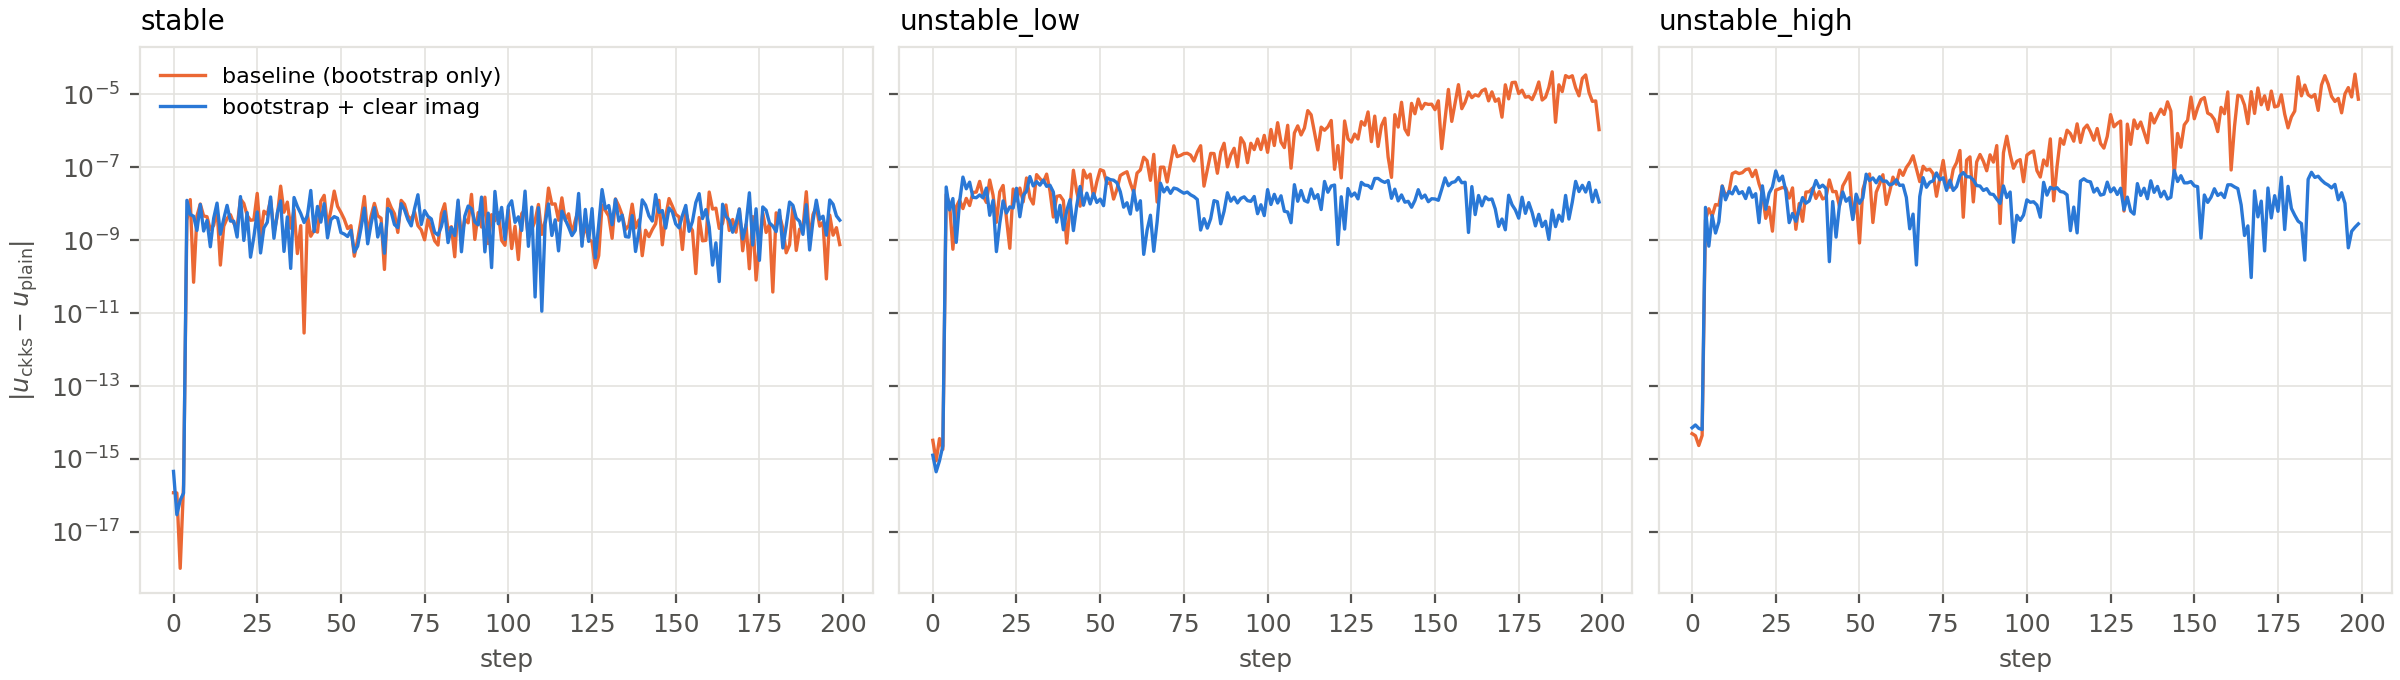
\includegraphics[width=\linewidth]{figures/u_error_clearimag.png}
\caption{Bootstrapping만 적용 (주황) vs.\ bootstrapping 후 허수부 제거 (파랑). 03 PT-CT, 200 step.}
\label{fig:cmp}
\end{figure}

\begin{table}[h]
\centering
\begin{tabular}{llrrrr}
\toprule
profile & 구현 & block 1 & block 10 & block 25 & block 49 \\
\midrule
stable        & 기존        & $1.3\times10^{-8}$ & $5.1\times10^{-9}$ & $6.9\times10^{-9}$ & $4.9\times10^{-9}$ \\
              & 허수부 제거 & $1.2\times10^{-8}$ & $2.3\times10^{-8}$ & $1.2\times10^{-8}$ & $1.3\times10^{-8}$ \\
unstable\_low  & 기존        & $1.8\times10^{-8}$ & $8.3\times10^{-8}$ & $1.7\times10^{-6}$ & $1.1\times10^{-5}$ \\
              & 허수부 제거 & $2.9\times10^{-8}$ & $1.3\times10^{-8}$ & $2.4\times10^{-8}$ & $3.8\times10^{-8}$ \\
unstable\_high & 기존        & $9.5\times10^{-9}$ & $4.5\times10^{-8}$ & $2.8\times10^{-7}$ & $3.6\times10^{-5}$ \\
              & 허수부 제거 & $7.9\times10^{-9}$ & $2.6\times10^{-8}$ & $1.3\times10^{-8}$ & $2.8\times10^{-9}$ \\
\bottomrule
\end{tabular}
\caption{Block별 최대 $|u_{\mathrm{ckks}}-u_{\mathrm{plain}}|$.}
\label{tab:fix}
\end{table}

허수부를 제거하면 unstable profile에서도 오차가 증가하지 않고 $10^{-8}$ 수준에 머문다.
이는 stable profile과 같은 수준이며, closed-loop 안정성에 의해 오차가 유계로 유지된다는 이론과 일치한다.
Plant state 오차도 세 profile 모두 $2\times10^{-8}$ 이하로 유지되었다.

\section{한계 및 남은 작업}
\begin{itemize}
\item 허수부 제거는 03 PT-CT에만 적용했다. 04 CT-CT에도 같은 수정이 필요하다 (04도 block당 $\approx1.19$배 증가를 보인다).
\item 수정 후 실험은 200 step만 수행했다. 기존 구현이 실패하던 360 step 이상의 장기 실행으로 재확인할 필요가 있다.
\item 04 CT-CT stable은 이 문제와 별개로 block 67에서 \texttt{Encode(): Scaling factor too small}로 중단되었다.
\item 로그에 기록되는 \texttt{epsilon\_u}는 block 내부의 국소 오차 ($u_{\mathrm{ckks}}-H z$, $z$는 복호화된 상태에서 시작한 정확한 전파)이며, 평문 제어기 대비 오차가 아니다. 본 문서의 비교는 \texttt{u\_ckks}$-$\texttt{u\_plain}을 사용했다.
\end{itemize}

\begin{thebibliography}{9}
\bibitem{kim} J.~Kim, ``Further methods for encrypted linear dynamic controllers utilizing re-encryption,'' arXiv:2307.16445, 2023.
\end{thebibliography}

\end{document}
